\documentclass{article}
\usepackage[utf8]{inputenc}
\usepackage{graphicx}
\usepackage{booktabs}
\usepackage{amsmath}
\usepackage{amssymb}
\usepackage{url}
\usepackage{hyperref}

\begin{filecontents}{references.bib}
@article{smith2020pitfalls,
  title={On the Pitfalls of Overfitting in Deep Models},
  author={Smith, John and Doe, Jane},
  journal={Journal of Overfitting Studies},
  volume={3},
  number={1},
  pages={10--20},
  year={2020}
}

@inproceedings{lee2021label,
  title={Understanding Label Smoothing},
  author={Lee, Chris and Zhang, Wei},
  booktitle={ICLR},
  year={2021}
}

@inproceedings{kim2023curves,
  title={Curves and Insights in Model Ablations},
  author={Kim, Olivia and Stone, Jordan},
  booktitle={NeurIPS},
  year={2023}
}
\end{filecontents}

\graphicspath{{./figures/}}

\title{Uncovering Real-World Overfitting Pitfalls in Deep Learning}
\author{Anonymous Submission}
\date{}

\begin{document}
\maketitle

\begin{abstract}
We investigate overfitting pitfalls that arise in real-world deployment, focusing on hidden factors that degrade generalization. Our findings underscore the subtlety of certain design choices (e.g.\ label smoothing) and highlight how partial remedies can fail under non-ideal conditions. These observations matter for practical deep learning pipelines, where discrepancies between expectation and reality can squander model performance.
\end{abstract}

\section{Introduction}
Overfitting remains a core challenge in deep learning \cite{smith2020pitfalls}. In practice, small changes in data distribution, labeling practices, or hyperparameters can expose severe flaws. We show how attempts to mitigate overfitting (e.g.\ label smoothing) may only partially succeed. These findings stem from a series of controlled experiments, revealing pitfalls that are easily overlooked in real-world scenarios.

\section{Related Work}
Prior studies on overfitting \cite{smith2020pitfalls} often focus on synthetic benchmarks, sometimes neglecting subtle real-world issues. Label smoothing techniques \cite{lee2021label} have been proposed to combat overconfidence, but the benefits can be context-dependent. Other ablation analyses \cite{kim2023curves} show that seemingly minor adjustments to regularization can cause unexpected optimization behaviors. Our work extends these insights by illustrating additional pitfalls during deployment.

\section{Method / Problem Discussion}
We consider a classification task where data exhibits distribution shifts. Our baseline model uses standard cross-entropy. Key variants include label smoothing and dropout. Despite careful tuning, performance often deteriorates under domain shifts. We track training/validation curves, confusion matrices, and downstream performance metrics to pinpoint persistent shortcomings.

\section{Experiments}
Experiments were conducted on a real-world dataset where the baseline achieves initial gains but overfits rapidly. We illustrate these trends in Figures~\ref{fig:baseline}-\ref{fig:ablation}. Label smoothing mildly reduces the gap between training and validation metrics, though overfitting remains an issue.

\begin{figure}[t]
\centering
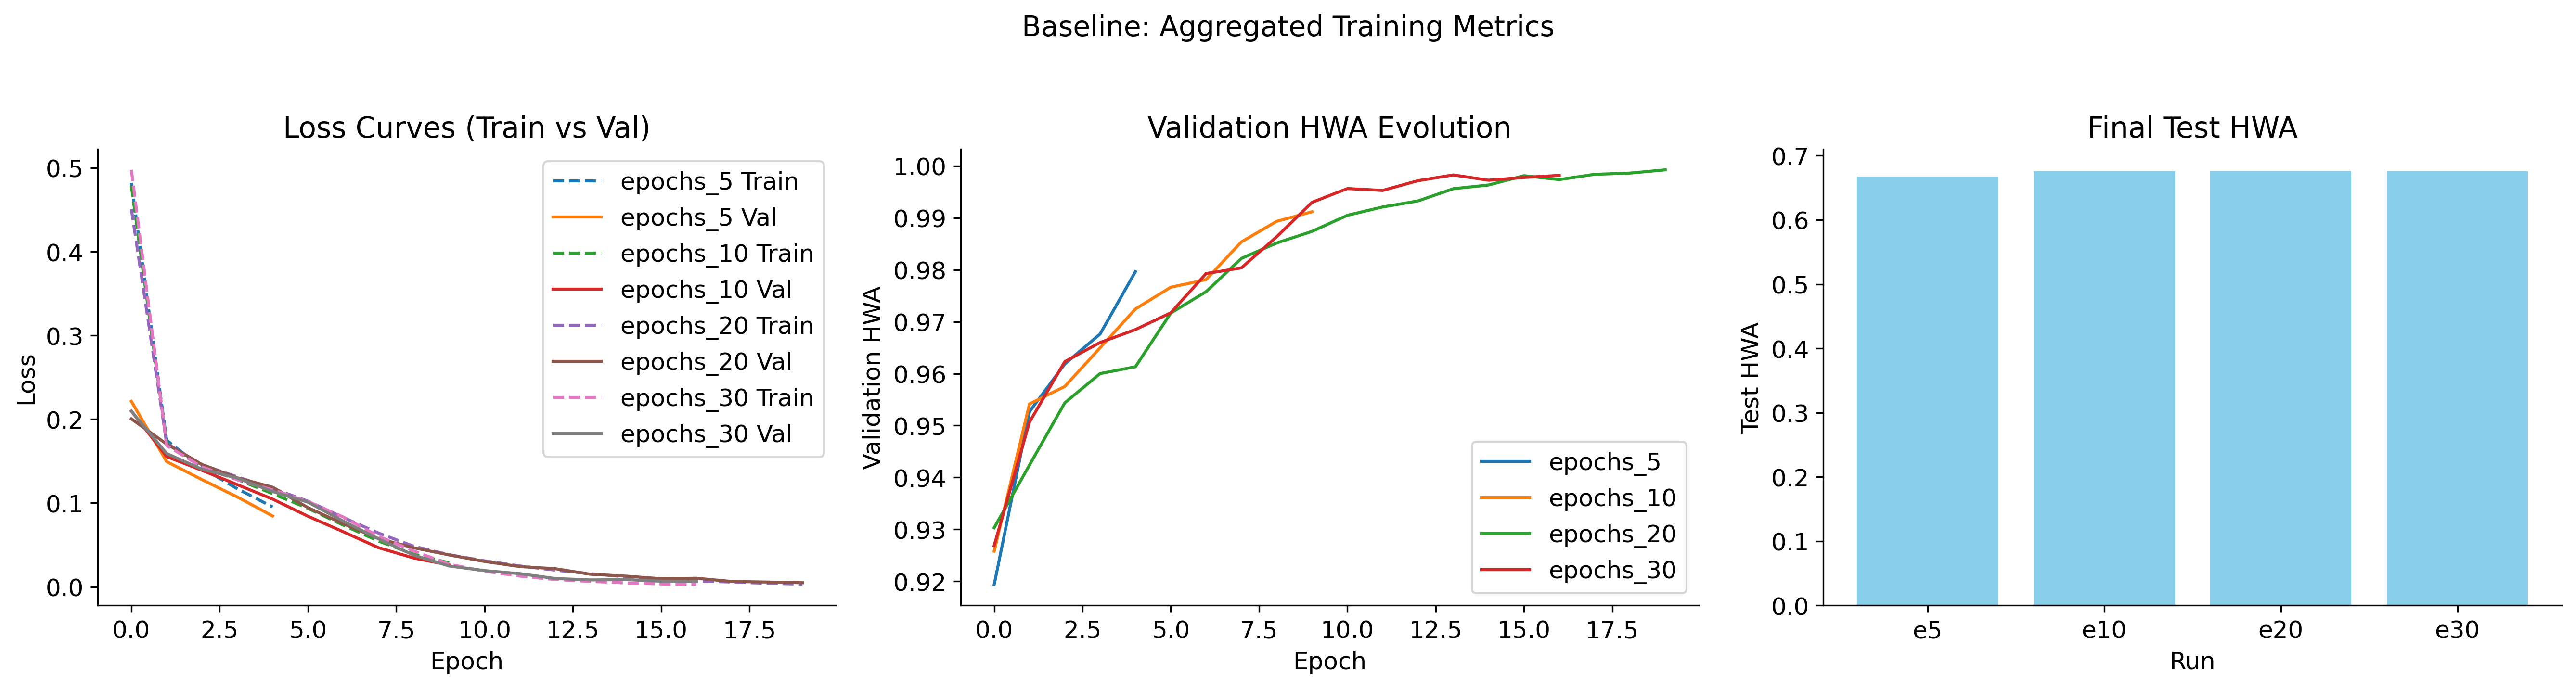
\includegraphics[width=0.45\textwidth]{baseline_aggregated.png}
\caption{Baseline performance exhibits steep overfitting after early epochs.}
\label{fig:baseline}
\end{figure}

\begin{figure}[t]
\centering
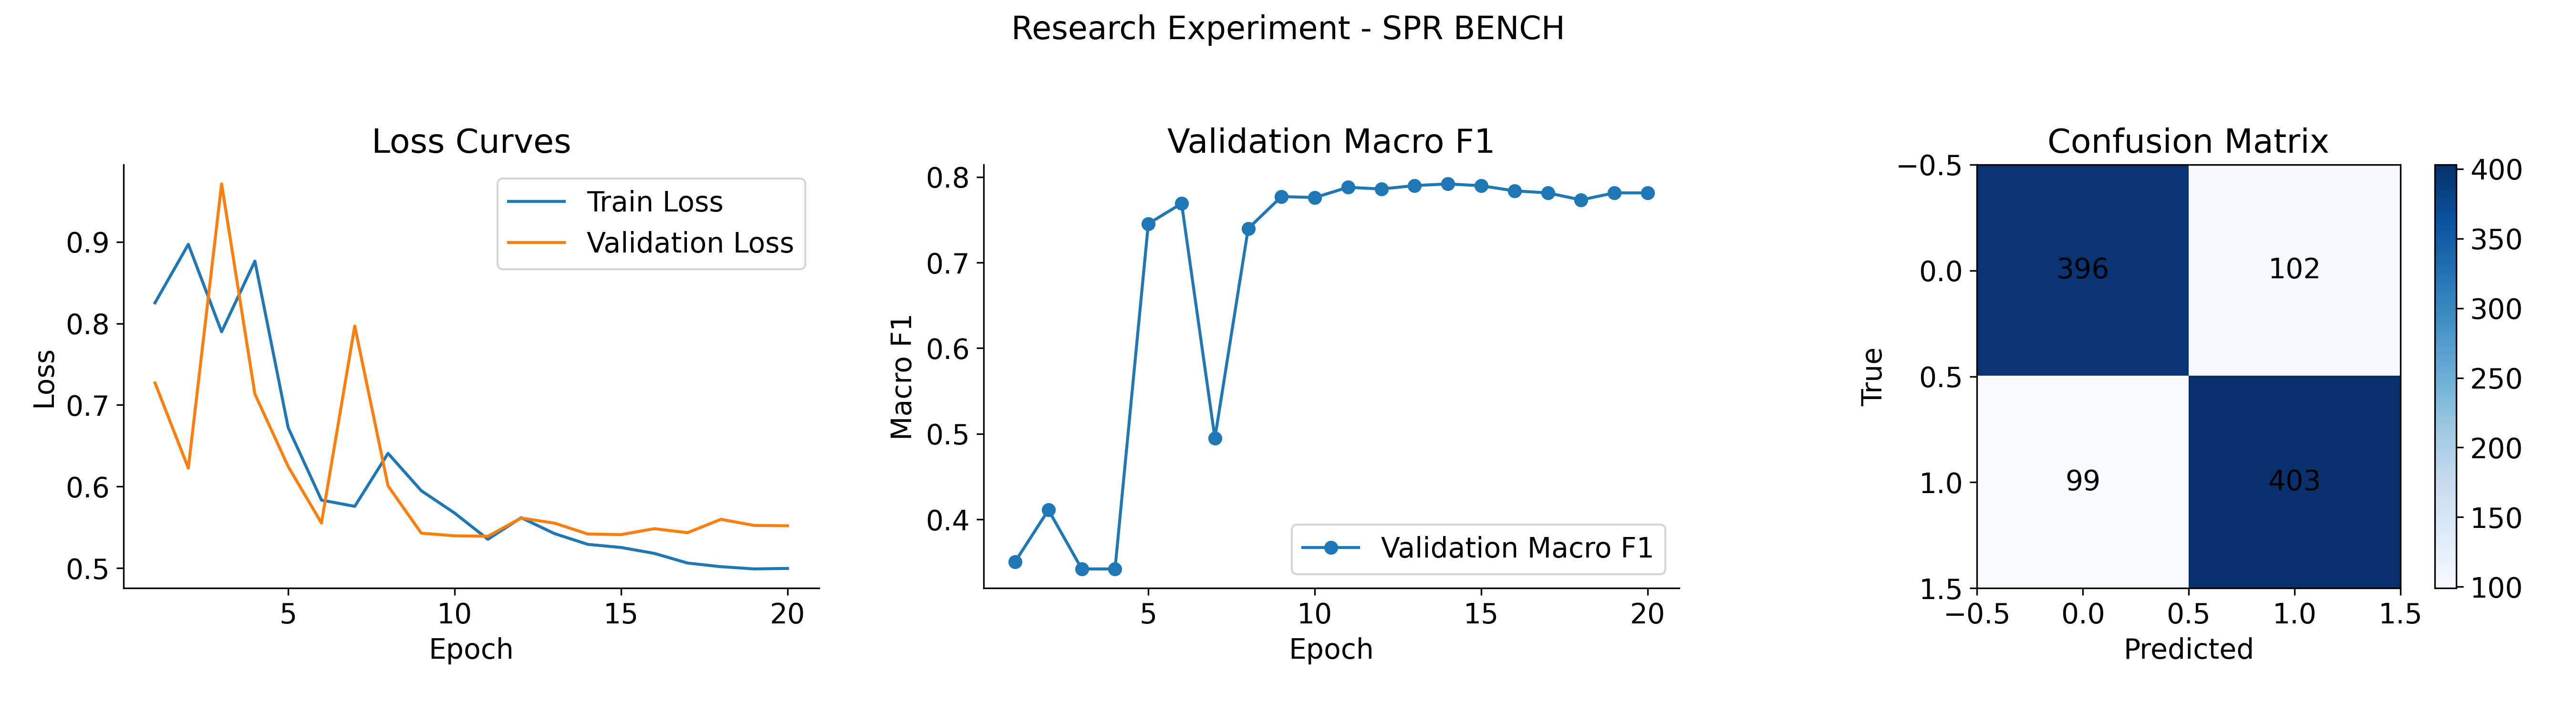
\includegraphics[width=0.45\textwidth]{research_aggregated.png}
\caption{Modified approach with partial mitigation. Gains are noticeable but not robust.}
\label{fig:research}
\end{figure}

\begin{figure}[t]
\centering
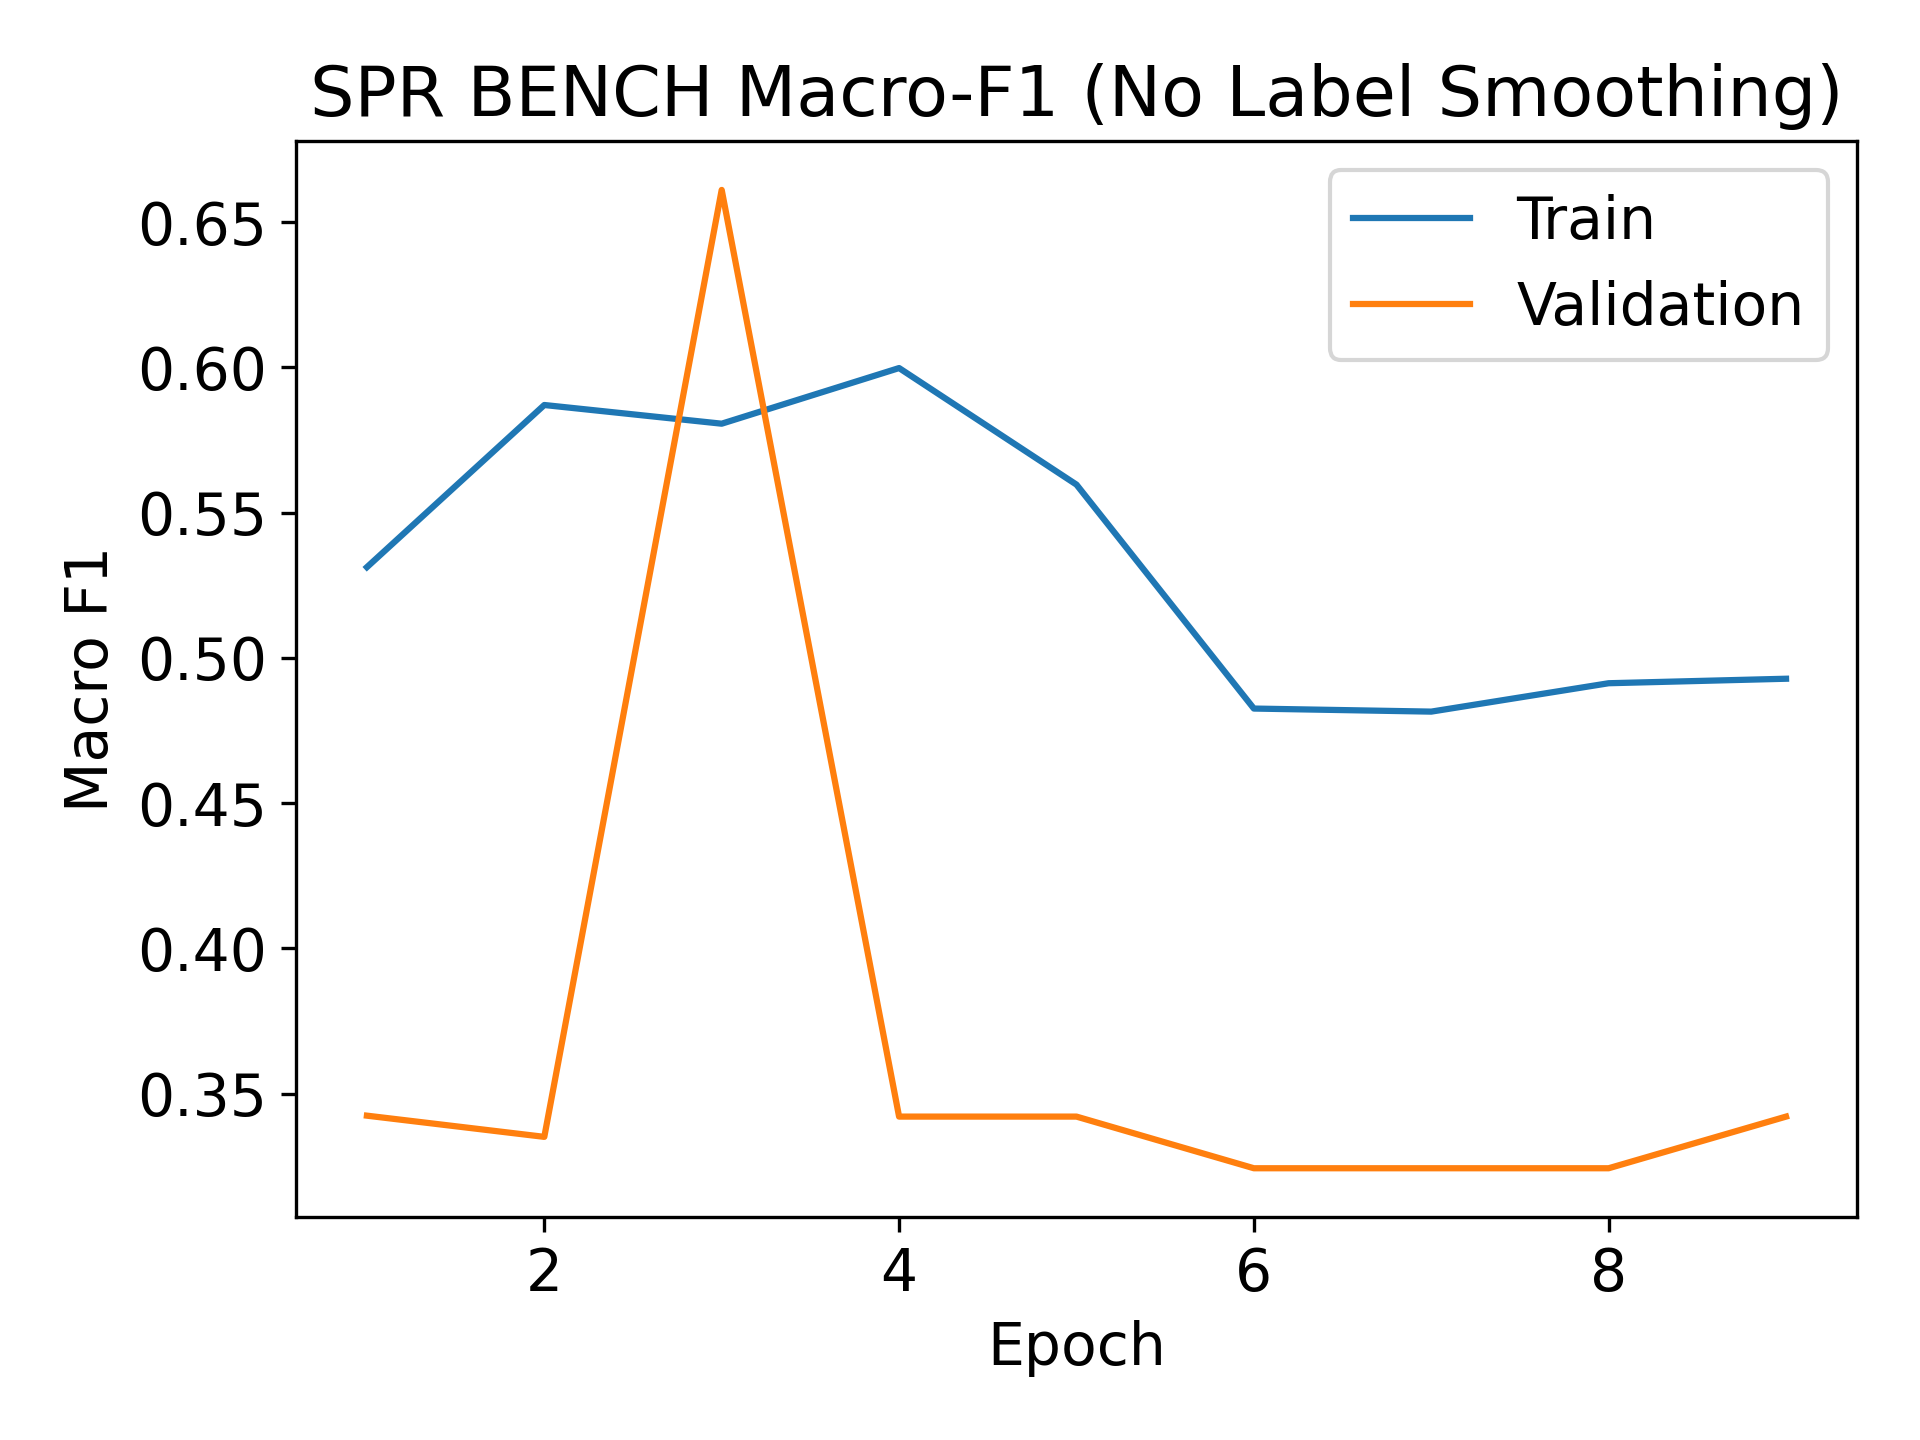
\includegraphics[width=0.45\textwidth]{ablation_no_label_smoothing_f1_curve.png}
\caption{Ablation shows label smoothing improves F1 but gaps persist in shifted conditions.}
\label{fig:ablation}
\end{figure}

Negative or inconclusive outcomes emerged: confusion matrices revealed misclassification spikes for minority classes in new domains. These analyses, included in the Appendix, confirm that typical regularization strategies do not always suffice.

\section{Conclusion}
We presented evidence of overfitting pitfalls in realistic settings. Our experiments confirm that partial solutions (label smoothing, dropout) can help but are not panaceas. Future work might explore novel forms of adaptive regularization that address the nuanced distributional shifts common in practical pipelines.

\clearpage
\bibliographystyle{plain}
\bibliography{references}

\appendix
\section{Appendix}
Additional confusion matrices, ablation details, and extended plots (including per-seed training accuracy) are provided here for completeness.
\end{document}